In this chapter, we present and discuss terms and known results in abstract, linear, complex and quaternion algebra which are key to understanding complex matrix representations of quaternionic linear maps.

\section{Rings, Fields, and Homomorphisms}
\begin{definition}[Ring] \label{def:ring}
	\emph{\cite{fraleigh}} A \emph{ring} is a set $R$ together with two binary operations $+$ (addition) and $\bigcdot$ (multiplication) defined on $R$ such that the following axioms are satisfied:
	\begin{varwidth}[t]{.9\textwidth}
	\centering
\begin{enumerate}
\item $R$ under $+$ is an abelian group.
\item Multiplication $\bigcdot$ is associative.
\item $\forall a,b,c \in R$ the left distributive law $a\bigcdot(b+c)=a\bigcdot b + a\bigcdot c$ and the right distributive law $(a+b)\bigcdot c = a\bigcdot c + b\bigcdot c$ hold.
\end{enumerate}
\end{varwidth}
\newline
\end{definition}

The first condition essentially means that a ring must form a group under addition $+$ (i.e., it's closed and associative under $+$, it contains an identity element and has an inverse for all its elements) and that addition is commutative \cite{fraleigh}. Rings in algebra are not to be confused with rings/tori (plural for torus) in geometry. The name \emph{ring} originally came from the word "Zahlring" (number ring) - a term introduced by D. Hilbert in 1897 - that may have something to do with cyclical behavior of powers of algebraic integers \cite{yrings}. Rings are one of the fundamental algebraic structures (groups and fields being the other two). Examples of rings are the integers $\mathbb{Z}$, the rational numbers $\mathbb{Q}$, the real numbers $\R$, the complex numbers $\CC$ and the quaternions $\HH$. 

Notice that a ring does not necessarily have a multiplicative identity. An example would be the ring of even integers $2\mathbb{Z}$ where the multiplicative identity 1 is not a member. If a ring does have a multiplicative identity, the multiplicative identity is called a \emph{unity} and the said ring is called a \emph{ring with unity} \cite{fraleigh}. In most of the rings we'll discuss, the multiplicative identity is 1. 

If the non-zero elements of a ring $R$ each have multiplicative inverses (i.e., for $a\in R$ and $a\neq 0$, $\exists a^{-1} \in R$ such that $aa^{-1}=a^{-1}a=1$) and are closed under ring multiplication, division becomes possible. Such a ring is called a \emph{division ring} or a \emph{skew field}.

\begin{definition}[Division Ring/Skew Field] \label{def:skewfield}
	\emph{\cite{fraleigh}} A \emph{division ring} or a \emph{skew field} is a ring whose non-zero elements form a group under multiplication.
\end{definition}

Note that a division ring does not necessarily have to be commutative under multiplication. A division ring that is commutative under multiplication is called a \emph{field}. Examples of division rings are the rational numbers $\mathbb{Q}$, the real numbers $\R$, the complex numbers $\CC$, and the quaternions $\HH$. The integers no longer form a division ring since the only non-zero element in $\mathbb{Z}$ that has a multiplicative inverse is the unity itself.

\begin{definition}[Field] \label{def:field}
	\emph{\cite{fraleigh}} A \emph{field} is a commutative division ring $R$, i.e., the non-zero elements of $R$ form an abelian group.
\end{definition}

Examples of fields are the rational $\mathbb{Q}$, real $\R$, and complex numbers $\CC$. The quaternions $\HH$ cannot form a field because they are, in fact, not commutative under multiplication. Rings, division rings, and fields can be summarized by the diagram shown in Figure \ref{fig:rings}.

\begin{figure}[H]
\centering
	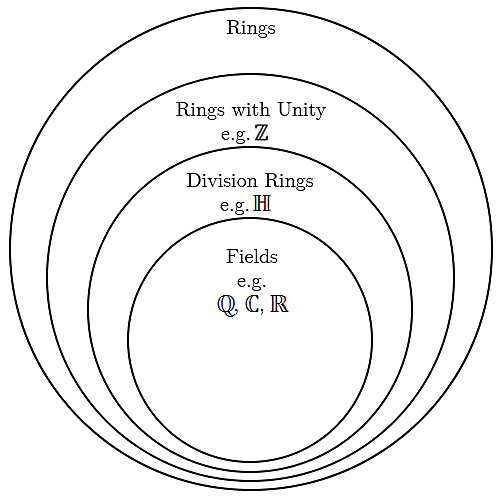
\includegraphics[scale=0.36]{rings_illustration}
	\caption{Diagram of Rings}
	\label{fig:rings}
\end{figure}

\begin{definition}[Homomorphism]
	\emph{\cite{fraleigh}} A map $\phi$ of a group $G$ into a group $G'$ is a \emph{homomorphism} if $\phi(ab)=\phi(a)\phi(b)$ $\forall a,b \in G$.
\end{definition}

A homomorphism is basically a structure-relating map that associates a binary operation in a group $G$ to a binary operation in another group $G'$. In other words, we say that the mapping \emph{preserves} the binary operation that gives $G$ its group structure. 

\begin{ex}
	Let $F$ be the additive group of continuous functions with domain $[0,1]$. The map $\sigma: F \rightarrow \R$ defined by $\sigma(f) = \int_{0}^{1} f(x) dx$ for $f \in F$ is a homomorphism since
	\begin{align*}
		\sigma(f+g) &= \int_{0}^{1} [f(x)+g(x)]dx \\
				  &= \int_{0}^{1} f(x)dx + \int_{0}^{1} g(x)dx \\
				  &= \sigma(f) + \sigma(g)
	\end{align*}
\end{ex}

\begin{ex} \label{ex:homomorph}
	Let $\CC$ be the field of complex numbers and $\Mr{2}$ the set of $2\times 2$ matrices. By Definition \ref{def:field}, this means that $\CC$ is a group under multiplication. The map $\phi: \CC \rightarrow \Mr{2}$ defined by 
	\begin{equation*}
		\phi(a+b\ib) = 
		\begin{pmatrix}
			a & -b \\
			b & a
		\end{pmatrix}
	\end{equation*}
	is a homomorphism (in fact, it is an \emph{injective homomorphism}, i.e., it is also one-to-one) since
	\begin{align*}
		\phi[(a+b\ib)(c+d\ib)] &= \phi[(ac-bd)+(bc+ad)\ib] \\
							   &=
							   \begin{pmatrix}
							   		ac-bd & -(bc+ad) \\
							   		bc+ad & ac-bd
							   \end{pmatrix} \text{ and,} \\
		\phi(a+b\ib)\phi(c+d\ib) &= 
								\begin{pmatrix}
									a & -b \\
									b & a
								\end{pmatrix}
								\begin{pmatrix}
									c & -d \\
									d & c
								\end{pmatrix} \\
								&= 
								\begin{pmatrix}
							   		ac-bd & -(bc+ad) \\
							   		bc+ad & ac-bd
							   \end{pmatrix}
	\end{align*}
	implying $\phi[(a+b\ib)(c+d\ib)] = \phi(a+b\ib)\phi(c+d\ib)$.
\end{ex}

\section{Vector Spaces and Linear Maps}

\begin{definition}[Vector Space] \label{vectspace}
	\emph{\cite{larson}} Let $V$ be a set on which two operations (vector addition and scalar multiplication) are defined and let $F$ be a field. If the listed axioms are satisfied $\forall \vec{u},\vec{v},\vec{w} \in V$ and $\forall c,d \in F$ (scalar), then $V$ is called a \emph{vector space} over the field $F$.
	\begin{varwidth}[t]{.35\textwidth}
\textbf{Scalar Multiplication:}
\begin{enumerate}
\item $c\vec{u} \in V$
\item $c(\vec{u}+\vec{v}) = c\vec{u}+c\vec{v}$
\item $(c+d)\vec{u} = c\vec{u}+d\vec{u}$
\item $c(d\vec{u}) = (cd)\vec{u}$
\item $1\vec{u} = \vec{u}$
\end{enumerate}
\end{varwidth}% <---- Don't forget this %
%\hspace{1em}% <---- Don't forget this %
\begin{varwidth}[t]{.65\textwidth}
\textbf{Vector Addition:} 
\begin{enumerate}
\item $\vec{u}+\vec{v} \in V$
\item $\vec{u}+\vec{v} = \vec{v}+\vec{u}$
\item $\vec{u}+(\vec{v}+\vec{w}) = (\vec{u}+\vec{v})+\vec{w}$
\item $V$ has a zero vector $\vec{0}$ such that $\forall \vec{u} \in V$, $\vec{u}+\vec{0} = \vec{u}$
\item $\forall \vec{u} \in V, \exists -\vec{u} \in V$ such that $\vec{u}+(-\vec{u}) = \vec{0}$.
\end{enumerate}
\end{varwidth}
\newline
\end{definition}

\newline
\newline

A vector space is basically any algebraic structure that follows a proper notion of vector addition and scalar multiplication, i.e., the latter operations satisfy the axioms in Definition \ref{vectspace}. A familiar example of a vector space would be the $n$-dimensional Euclidean space over the field $\R$ ($\R^n$) where we represent vectors as $n$-tuples with components in $\R$. In $\R^2$ and $\R^3$, we commonly visualize vectors as arrows in space with magnitude and direction. However, there are other vector spaces that cannot be visualized just as easily, such as the vector space of polynomials of degree $n$ ($P(n)$) \cite{3b1b} \cite{larson}. The polynomials form a vector space because they have a notion of vector addition (addition of like terms) and scalar multiplication (multiplication by a constant) \cite{3b1b} \cite{larson}. Another vector space which will be of great importance throughout the discussion is the \emph{complex vector space} which is simply the Euclidean vector space over the field $\CC$ ($\CC^n$).

\begin{definition}[Linear Map/ Linear Transformation] \label{linmapdef}
	\emph{\cite{larson}} Let $V, W$ be vector spaces over the field $F$. The function $L: V \rightarrow W$ is called a \emph{linear map/ linear transformation} of $V$ into $W$ when the following properties are true $\forall u,v \in V$ and $\forall c \in F$:
	\newline\newline
	\begin{enumerate}
		\item L(u+v) = L(u)+L(v)
		\item L(cu) = cL(u)
	\end{enumerate}
\end{definition}

 We can view Property 1 of Definition \ref{linmapdef} as having the linear map $L$ commute with vector addition, i.e., the image of the vector sum is the sum of the images. Property 2 of Definition \ref{linmapdef} is interpreted as having the linear map commute with scalar multiplication. Notice that Definition \ref{vectspace} only considers scalar multiplication in the context of fields. In the case of non-commutative skew fields like the quaternions, we will have to specify the type of scalar multiplication in the vector space, i.e., either right or left scalar multiplication \cite{stack}. If we only consider right scalar multiplication in Definition \ref{vectspace}, we have what is called a \emph{right vector space} (provided that all the axioms are satisfied given the choice of scalar multiplication) \cite{stack}. An example of a right vector space is the \emph{right quaternionic vector space}. We will later see that we can still define linear maps in quaternions provided that we only consider right vector spaces \cite{stack} \cite{aslaksen}.

We know from linear algebra that every linear transformation/linear map $L: V \rightarrow W$ (where $V$ and $W$ are vector spaces of dimension $n$ and $m$ respectively) has an $m\times n$ matrix representation \cite{larson}. Thus, we can essentially interchange the terms \emph{matrix} and \emph{linear map} throughout the discussion. 

\section{Complex Matrices}

Our discussions regarding quaternionic linear maps/matrices will mostly revolve around extending properties and definitions that already hold for complex matrices. We begin by extending properties and definitions that already hold for real matrices to complex matrices.

\emph{Complex Matrices} are matrices that have entries in $\CC$. They are linear maps $L_{\CC}: V \rightarrow W$ where $V$ and $W$ are \emph{complex vector spaces}. Since its entries are complex numbers, we can take the conjugate of each of its entries. We call the resulting matrix a \emph{conjugate matrix}.
\newpage
\begin{definition}[Conjugate Matrix]
	\emph{\cite{stamaria}} A \emph{conjugate matrix} is a matrix $\bar{E}$ obtained from a complex matrix $E \in \Mc{n}$, where $\Mc{n}$ is the set of all $n \times n$ complex matrices,  by taking the complex conjugate of every entry of $E$.
\end{definition}

\begin{ex}
	Take $E = $
	\begin{pmatrix} 
	-\frac{13}{17}+\frac{16}{17}\ib & -\frac{8}{17}+\frac{2}{17}\ib \\
	\frac{16}{17}-\frac{4}{17}\ib & \frac{19}{17}+\frac{8}{17}\ib
	\end{pmatrix}. 
	Then $\overline{E} = $
	\begin{pmatrix} 
		-\frac{13}{17}-\frac{16}{17}\ib & -\frac{8}{17}-\frac{2}{17}\ib \\
		\frac{16}{17}+\frac{4}{17}\ib & \frac{19}{17}-\frac{8}{17}\ib
	\end{pmatrix}
\end{ex}

Operations and properties that we know hold for real matrices like matrix addition and multiplication, elementary row operations, matrix inverse, and the determinant still hold for complex matrices \cite{aslaksen}.

\begin{definition}[Complex Determinant]
	\emph{\cite{larson}} The \emph{Complex Determinant}, denoted by $\ccdet$, of an $n\times n$ complex matrix $E$ is defined by,
	$$\ccdet(E) = |E| = \sum_{j=1}^{n} a_{ij}c_{ij}$$
	where $c_{ij} = (-1)^{i+j}M_{ij}$ and $M_{ij}$ is the determinant of the matrix obtained by deleting the $i^{th}$ row and $j^{th}$ column.
\end{definition}

Notice that, computationally, the complex determinant is no different from the real determinant. The only difference is that computing for the determinant of a complex matrix will give us a complex number.

\begin{theorem} \label{detbar}
	For a matrix $E \in \Mc{n}$, $\ccdet(\bar{E}) = \overline{\ccdet(E)}$.
\end{theorem}

\begin{proof}
	We prove by mathematical induction. 
	\newline
	Let $\Mc{n}$ denote the set of all $n\times n$ complex matrices. Let $n = 2$ and take $E$ = 
	\begin{pmatrix}
		\bar{a} & \bar{b} \\
		\bar{c} & \bar{d}
	\end{pmatrix}. Then,  
	$\ccdet(\bar{E})$ & =
	\begin{vmatrix}
		\bar{a} & \bar{b} \\
		\bar{c} & \bar{d}
	\end{vmatrix} $= \overline{ad} - \overline{bc} = \overline{ad-bc} = \overline{\ccdet(E)}$
	\newline
	\newline
	Suppose $\overline{\ccdet(E)} = \ccdet(\bar{E})$ holds for $E \in \Mc{k}$ for some $k\geq 2$ ($\ast$).
	\newline
	Let $X \in \Mc{k+1}$. Then, $$\overline{\ccdet(X)} = \overline{\sum_{j=1}^{k+1} a_{ij}c_{ij}} = \sum_{j=1}^{k+1} \overline{a_{ij}}\text{ }\overline{c_{ij}}$$
	\newline
	Note that $\overline{c_{ij}} = (-1)^{i+j}\overline{M_{ij}}$ where $\overline{M_{ij}}$ is the determinant of the $k\times k$ matrix obtained by deleting the $i^{th}$ row and the $j^{th}$ column of the original matrix.
	\newline
	By ($\ast$), $\overline{M_{ij}}$ is the determinant of a $k\times k$ conjugate matrix. Thus, we see that we are computing for the determinant of a $(k+1)\times (k+1)$ conjugate matrix. 
\end{proof}
\newline
\newline
Theorem \ref{detbar} states that computing for the determinant commutes with conjugation, i.e., the determinant of the conjugate matrix is the conjugate of the determinant. 

\begin{definition}[Coninvolutory Matrix]
	\emph{\cite{stamaria}} A matrix is said to be \emph{coninvolutory} if $E\bar{E} = I_n$ for $E \in \Mc{n}$ where $\Mc{n}$ denotes the set of all $n \times n$ complex matrices.
\end{definition}	

	By manipulation, we obtain $E^{-1} = \bar{E}$. Hence, a matrix whose inverse is its own conjugate matrix is a coninvolutory matrix. 
\begin{ex}
	Consider the complex matrix, $E = $
	\begin{pmatrix} 
	-\frac{13}{17}+\frac{16}{17}\ib & -\frac{8}{17}+\frac{2}{17}\ib \\
	\frac{16}{17}-\frac{4}{17}\ib & \frac{19}{17}+\frac{8}{17}\ib
	\end{pmatrix}
	
	We see that 
	\begin{align*}
	E\bar{E} &=  
		\begin{pmatrix} 
		-\frac{13}{17}+\frac{16}{17}\ib & -\frac{8}{17}+\frac{2}{17}\ib \\
		\frac{16}{17}-\frac{4}{17}\ib & \frac{19}{17}+\frac{8}{17}\ib
		\end{pmatrix}
		\begin{pmatrix} 
		-\frac{13}{17}-\frac{16}{17}\ib & -\frac{8}{17}-\frac{2}{17}\ib \\
		\frac{16}{17}+\frac{4}{17}\ib & \frac{19}{17}-\frac{8}{17}\ib
		\end{pmatrix} \\
		&= \frac{1}{17}\frac{1}{17}
		\begin{pmatrix}
		-13+16\ib & -8+2\ib \\
		16-4\ib & 19+8\ib
		\end{pmatrix}
		\begin{pmatrix}
		-13-16\ib & -8-2\ib \\
		16+4\ib & 19-8\ib
		\end{pmatrix} \\
		&=
		\frac{1}{289}
		\begin{pmatrix}
		289 & 0 \\
		0 & 289
		\end{pmatrix} \\
		&=
		\begin{pmatrix}
		1 & 0 \\
		0 & 1
		\end{pmatrix} \\
		&= I_2
	\end{align*}
We see that $E$ is a coninvolutory matrix. \textit{Remark:} We've obtained $E$ using the factorization provided in Theorem 2.3 found in \cite{stamaria}. 

\end{ex}
	\textit{Remark.} If we take the concept of coninvolutory matrices in the context of real matrices, we get $EE = E^2 = I_n$ since for any $n\times n$, $E = \overline{E}$. This is what we call an \emph{Involutory Matrix}, i.e.,  a matrix whose inverse is itself. 

\begin{definition}[Involutory Matrix]
	An $n \times n$ real matrix $X$ is called an \emph{involutory matrix} if $X^2 = I_n$ where $I_n$ is the $n \times n$ identity matrix.
\end{definition}

	Because linear maps that represent a $180\degree$ rotation or a reflection are of order 2 (i.e. applying their associated actions twice on a point/vector leaves the point/vector unchanged), they are involutory matrices. 
\begin{ex}
	Take the rotation matrix $\Rx{R}{x}{\alpha}$ in Chapter 1. If $\alpha = \pi$, we have a rotation matrix that represents a $180\degree$ rotation given by,
	\begin{align*}
		\Rx{R}{x}{\pi} = 
			\begin{pmatrix}
				1 & 0 & 0 & 0 \\
				0 & \cos{\pi} & -\sin{\pi} & 0 \\
				0 & \sin{\pi} & \cos{\pi} & 0 \\
				0 & 0 & 0 & 1
			\end{pmatrix} 
			=
			\begin{pmatrix}
				1 & 0 & 0 & 0 \\
				0 & -1 & 0 & 0 \\
				0 & 0 & -1 & 0 \\
				0 & 0 & 0 & 1
			\end{pmatrix}
	\end{align*}.
	We now see that,
	\begin{align*}
		(\Rx{R}{x}{\pi})^2 = 
			\begin{pmatrix}
				1 & 0 & 0 & 0 \\
				0 & -1 & 0 & 0 \\
				0 & 0 & -1 & 0 \\
				0 & 0 & 0 & 1
			\end{pmatrix}
			\begin{pmatrix}
				1 & 0 & 0 & 0 \\
				0 & -1 & 0 & 0 \\
				0 & 0 & -1 & 0 \\
				0 & 0 & 0 & 1
			\end{pmatrix}
			=
			\begin{pmatrix}
				1 & 0 & 0 & 0 \\
				0 & 1 & 0 & 0 \\
				0 & 0 & 1 & 0 \\
				0 & 0 & 0 & 1
			\end{pmatrix}
			= I_4
	\end{align*}
\end{ex}
\begin{definition}[Skew-Coninvolutory Matrix]
	\emph{\cite{stamaria}} A matrix is said to be \emph{skew-coninvolutory} if $E\bar{E} = -I_n$ for $E \in \Mc{n}$.
\end{definition}

	We see that a matrix whose inverse is the negative of its own conjugate matrix is a skew-coninvolutory matrix. 

	\textit{Remark.} If we take this in the context of real matrices, we get $EE = E^2 = -I_n$. Notice how this closely resembles a property of the complex number $\ib$, i.e., $\ib^2 = -1$. In fact, we have a special name for these linear maps. We call them \emph{complex structures} \cite{wolfram}. 

	\begin{definition}[Complex Structure] \label{def:compstruct}
	\emph{\cite{wolfram}} A \emph{complex structure} of a vector space $V$ is defined by the linear map (linear transformation) $J: V \rightarrow V$ such that $J^2 = -I$, where $I$ is the identity map. \cite{wolfram} 
\end{definition}
 \newline
 \newline
 \textit{Remark.} If a vector space $V$ has a complex structure (i.e. if we can define a complex structure in the vector space), it means that $V$ can essentially "mimic" a complex vector space \cite{jwr}. 
 To see how this works, observe Example \ref{ex:complexstruct}.

 \begin{ex} \label{ex:complexstruct}
 	The matrix $J = $
 	\begin{pmatrix}
 		0 & -1 \\
 		1 & 0
 	\end{pmatrix}
 	gives a complex structure in $\R^2$ since
 	\begin{align*}
 		J^2 = 
 		\begin{pmatrix}
 			0 & -1 \\
 			1 & 0
 		\end{pmatrix}
 		\begin{pmatrix}
 			0 & -1 \\
 			1 & 0
 		\end{pmatrix}
 		 = 
 		\begin{pmatrix}
 			-1 & 0 \\
 			0 & -1
 		\end{pmatrix}
 		 = -I_2.
 	\end{align*}
 	If we can think of $a+b\ib \in \CC$ as a 2-dimensional vector $\vec{v} = \vectC{a}{b}$ and multiply $\vec{v}$ by $J$, we get, 
 	\begin{align*}
	 	\begin{pmatrix}
	 			0 & -1 \\
	 			1 & 0
	 	\end{pmatrix}
	 	\vectC{a}{b} = \vectC{-b}{a}
 	\end{align*}
 	which corresponds to the product of $\ib$ and $a+b\ib$, $-b+a\ib$.
 \end{ex}

 There are vector spaces in which we cannot define a complex structure. For instance, the vector space $\R^1$ or simply $\R$. Since this is a 1-dimensional vector space, we have $1\times 1$ matrices to represent linear maps $L_1: \R \rightarrow \R$. Linear maps like $L_1$ are identical to scalar multiplication. Since there is no element $x \in \R$ such that $x^2 = -1$, we cannot define a complex structure in $\R$. 

 We can observe a pattern in the dimensions of the vector spaces where a complex structure can be defined. We see that only vector spaces (specifically real vector spaces) with even dimensions can have a complex structure defined. This is proven in the context of skew-coninvolutory complex matrices as shown in Theorem \ref{dnc}.

\begin{theorem} \label{dnc}
	\emph{\cite{stamaria}} Let $\mathscr{D}_{n}(\CC)$ denote the set of all $n \times n$ skew-coninvolutory complex matrices. Then $\mathscr{D}_{n}(\CC)$ is empty when $n$ is odd.
\end{theorem}

\begin{proof}
	If $E \in \mathscr{D}_{n}(\CC)$ then $E\bar{E} = -I_n$. \newline Taking the determinant of both sides, 
	\begin{align*}
		\ccdet(E\bar{E}) &= \ccdet(-I_n) \\
		\ccdet(E)\ccdet(\bar{E}) &= (-1)^n \\
		\ccdet(E)\overline{\ccdet(E)} &= (-1)^n \text{, by Theorem \ref{detbar}} \\
		|\ccdet(E)|^2 &= (-1)^n \text{, since $\ccdet$ yields a complex number.}
	\end{align*}
	Since $|\ccdet(E)|^2 > 0$, $(-1)^n > 0$. Hence, $n$ must be even.
\end{proof}
\newline
\newline
\textit{Remark.} Theorem \ref{dnc} puts a restriction on the dimension of complex matrices that are skew-coninvolutory. In the context of real matrices, this means that $E^2 = -I_n$ only holds if $E$ is a $2n\times 2n$ real matrix, i.e., a complex structure only exists for real matrices with even dimensions. 
\begin{ex} 
We see that in the $1\times 1$ case, $\bar{\ib} = -\ib$ but $\ib\bar{\ib} = -\ib^2 = 1 \neq -1$. Whereas in the $2\times 2$ case, consider $E = 
\begin{pmatrix}
	0 & \ib \\
	-\ib & 0
\end{pmatrix}$.
Then $E\bar{E} = 
\begin{pmatrix}
	0 & \ib \\
	-\ib & 0
\end{pmatrix}
\begin{pmatrix}
	0 & -\ib \\
	\ib & 0
\end{pmatrix}  = 
\begin{pmatrix}
	-1 & 0 \\
	0 & -1
\end{pmatrix}$.
\end{ex} 
We will see more manifestations of Theorem \ref{dnc} in later discussions especially when we represent complex matrices as real matrices.

\section{Basics of Quaternion Algebra}

In this section, we introduce properties and operations associated with quaternions such as addition, multiplication, conjugation, norm, and inverse.

\begin{definition}[Quaternion] \label{quatdef}
	\emph{\cite{stamaria}} The four-dimensional algebra of \emph{Quaternions}, denoted by $\HH$, is generated by the basis elements $\{1,\ib,\jb,\kb\}$ such that $\ib^2 = \jb^2 = \kb^2 = \ib \jb \kb = -1$. $\HH := \{\quat{a}{b}{c}{d} | a,b,c,d \in \R\}$. 
\end{definition}

Examples of quaternions are $1+2\ib+3\jb+4\kb$, $-2+5\ib-6\kb$, and $3\ib-\frac{1}{2}\jb+\sqrt{2}\kb$. As seen in Chapter 1, we can also write a quaternion $\quat{a}{b}{c}{d}$ as an ordered pair $(a,\vec{v})$ where $a$ is a scalar and $\vec{v}$ is a 3-dimensional vector corresponding to the coefficients of $\ib, \jb$ and $\kb$ respectively, i.e., the vector $(b,c,d)$. For instance, the quaternion $-2+5\ib-6\kb$ can be written as $(-2,(5,0,-6))$ and the quaternion $3\ib-\frac{1}{2}\jb+\sqrt{2}\kb$ can be written as $(0,(3,-\frac{1}{2},\sqrt{2}))$. We call a quaternion whose scalar part $a = 0$, a \emph{pure quaternion} \cite{lerios} \cite{mathoma}. Notice that $\CC \subseteq \HH$ since a quaternion becomes a complex number if $c,d = 0$.
\newpage
\subsection{Addition and Multiplication}

\textbf{Addition.} Adding quaternions is straightforward and follows component-wise addition.
\begin{definition}[Quaternion Addition] \label{quatp}
 \emph{\cite{lerios}} For quaternions $q_1 = a_1 + b_1\ib + c_1\jb + d_1\kb$ and $q_2 = a_2 + b_2\ib + c_2\jb + d_2\kb$, $$q_1+q_2 = (a_1+a_2) + (b_1+b_2)\ib + (c_1+c_2)\jb + (d_1+d_2)\kb.$$ 
\end{definition}
Alternatively, if $q_1 = (a_1,\vec{v_1})$ and $q_2 = (a_2,\vec{v_2})$ where $\vec{v_1}$ and $\vec{v_2}$ are $(b_1,c_1,d_1)$ and $(b_2,c_2,d_2)$ respectively, then $$(a_1,\vec{v_1})+(a_2,\vec{v_2}) = (a_1+a_2,\vec{v_1}+\vec{v_2})$$ 

The quaternions form an \emph{abelian group} under addition (i.e., they form a commutative group under addition) because: (1) quaternion addition is associative, (2) the additive identity 0 is a quaternion, (3) the additive inverse of a quaternion $q$ is $-q$ which is also a quaternion, and (4) quaternion addition is commutative since the scalars $a,b,c$ and $d$ are in $\R$. 

\noindent\textbf{Multiplication.} Quaternion multiplication is governed by Definition \ref{quatdef}, where $\ib^2 = \jb^2 = \kb^2 = \ib \jb \kb = -1$. We can then derive the following: 
\begin{align*} 
	\jb\kb &= \ib & \kb\jb &= -\ib \\
	\kb\ib &= \jb & \ib\kb &= -\jb \\
	\ib\jb &= \kb & \jb\ib &= -\kb
\end{align*}

It can be useful to remember the multiplication of $\ib, \jb$ and $\kb$ using Figure \ref{fig:quatxvis}. We see that going about the circle clockwise starting at $\ib$ and going to $\jb$ gives us a positive $\kb$. On the other hand, going about the circle counter-clockwise starting at $\kb$ and going to $\jb$ gives us a negative $\ib$.

\begin{figure}[H]
	\centering
	\subfloat[Positive]{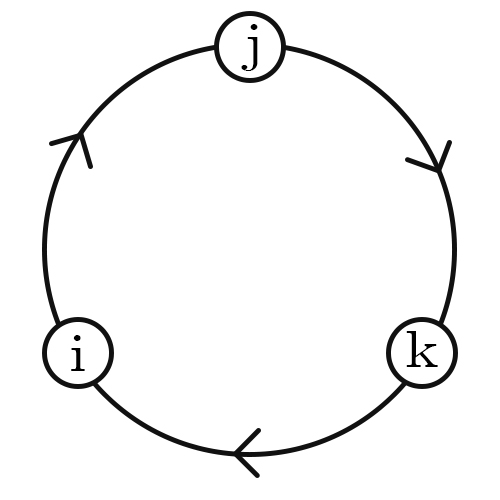
\includegraphics[scale=0.35]{positive.jpg}\label{fig:posvis}}
	\subfloat[Negative]{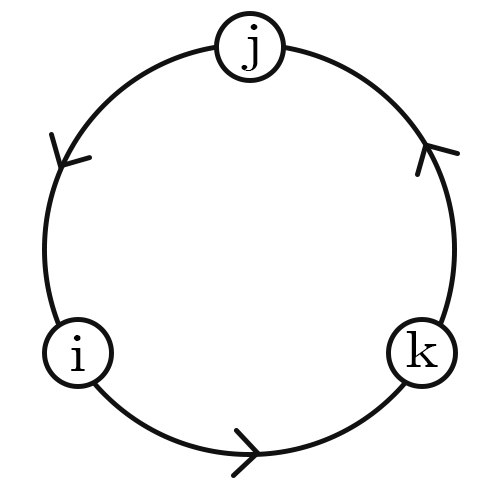
\includegraphics[scale=0.35]{negative.jpg}\label{fig:negvis}}
	\caption{Visualizing the multiplication of $\ib, \jb$ and $\kb$}
	\label{fig:quatxvis}
\end{figure}

From elements $\ib,\jb$ and $\kb$ alone, we can already see that the quaternions are not commutative under multiplication. However, quaternion multiplication is associative \cite{lerios}. Furthermore, quaternions commute with a scalar in $\R$ \cite{lerios}

\begin{definition}[Quaternion Multiplication] \label{quatx}
	\emph{\cite{lerios}} For quaternions $q_1 = a_1 + b_1\ib + c_1\jb + d_1\kb$ and $q_2 = a_2 + b_2\ib + c_2\jb + d_2\kb$, 
	\begin{align*}
		q_1q_2 &= (a_1a_2 - b_1b_2 - c_1c_2 - d_1d_2) + (a_1b_2 + b_1a_2 + c_1d_2 - d_1c_2)\ib \\
			   &+ (a_1c_2 - b_1d_2 + c_1a_2 + d_1b_2)\jb + (a_1d_2 + b_1c_2 - c_1b_2 + d_1a_2)\kb
	\end{align*}
\end{definition}

\begin{ex} \label{ex:quatx}
	Take the quaternions $q_1 = 1+2\ib+3\jb+4\kb$ and $q_2 = -2+5\ib-6\kb$. Using the formula given by Definition \ref{quatx}, we have,
	\begin{align*}
		q_1 q_2 &= [(1)(-2)-(2)(5)-(3)(0)-(4)(-6)] + [(1)(5)+(2)(-2)+(3)(-6)-(4)(0)]\ib \\
		&+[(1)(0)-(2)(-6)+(3)(-2)+(4)(5)]\jb + [(1)(-6)+(2)(0)-(3)(5)+(4)(-2)]\kb \\
		&= 12 - 17\ib + 26\jb - 29\kb.
	\end{align*}
\end{ex}

\textit{Remark.} Alternatively, by viewing quaternions as ordered pairs $q_1 = (a_1,\vec{v_1})$ and $q_2 = (a_2,\vec{v_2})$ we can restate Definition \ref{quatx} as,
\begin{equation} \label{eq:qvectx}
	q_1 q_2 = (a_1a_2 - \vec{v_1}\bigcdot\vec{v_2},\text{ } a_1\vec{v_2}+a_2\vec{v_1}+\vec{v_2}\times\vec{v_1})
\end{equation}
where $\vec{v_1}\bigcdot\vec{v_2}$ and $\vec{v_2}\times\vec{v_1}$ are the vector \emph{dot product} and \emph{cross product} respectively \cite{lerios} \cite{mathoma}.

\begin{ex}
	We can compute for the product of the quaternions given in Example \ref{ex:quatx} using Equation \ref{eq:qvectx}. For $q_1 = (1,(2,3,4))$ and $q_2 = (-2,(5,0,-6))$, we have
	\begin{align*}
		q_1 q_2 &= ((1)(-2)-(10-24),\text{ }(5,0,-6)-2(2,3,4)+(-18,32,-15)) \\
		&= (12,(-17,26,-29))
	\end{align*}
\end{ex}

\begin{theorem} \label{theorem:distquat}
	For quaternions $q, p$ and $r$, $q(p+r) = qp+qr$ and $(p+r)q = pq + rq$, i.e., the left and right distributive laws hold.
\end{theorem}

\begin{proof}
	Let $q = (q_0,\vec{q})$, $p = (p_0,\vec{p})$, and $r = (r_0,\vec{r}) \in \HH$. Then,
	\begin{align*}
		q(p+r) &= (q_0,\vec{q})[(p_0,\vec{p})+(r_0,\vec{r})] \\
			   &= (q_0,\vec{q})((p_0+r_0),\vec{p}+\vec{r}) \text{ by Definition \ref{quatp}} \\
			   &= (q_0(p_0+r_0)-\vec{q}\bigcdot(\vec{p}+\vec{r}), q_0(\vec{p}+\vec{r})+(p_0+r_0)\vec{q}+(\vec{p}+\vec{r})\times\vec{q}\text{ })\\
			   &\text{by Definition \ref{quatx}} \\
			   &= (q_0p_0+q_0r_0-\vec{q}\bigcdot\vec{p}-\vec{q}\bigcdot\vec{r}, q_0\vec{p} + q_0\vec{r} + p_0\vec{q}+ r_0\vec{q} + \vec{p}\times\vec{q} + \vec{r}\times\vec{q}\text{ }) \\
			   &\text{since the distributive laws hold for dot products and cross products \cite{larson}.}\\
			   &= ((q_0p_0-\vec{q}\bigcdot\vec{p})+(q_0r_0-\vec{q}\bigcdot\vec{r}), (q_0\vec{p}+ p_0\vec{q}+ \vec{p}\times\vec{q}) + (q_0\vec{r} + r_0\vec{q} + \vec{r}\times\vec{q})\text{ }) \\
			   &=(q_0p_0-\vec{q}\bigcdot\vec{p},q_0\vec{p}+ p_0\vec{q}+ \vec{p}\times\vec{q}\text{ }) + (q_0r_0-\vec{q}\bigcdot\vec{r},q_0\vec{r} + r_0\vec{q} + \vec{r}\times\vec{q}\text{ }) \\
			   &=qp + qr.
	\end{align*}
	The right distributive law can also be proven in a similar manner.
\end{proof}
\newline
\newline
\textit{Remark.} Since (1) the quaternions form an abelian group under quaternion addition, (2) quaternion multiplication is associative and (3) the left and right distributive laws hold, by Definition \ref{def:ring} the set of quaternions $\HH$ forms a ring.

\subsection{Other Operations and Properties}

\begin{definition}[$\HH$-Conjugate] \label{hconj}
	\emph{\cite{stamaria}}The $\HH$-Conjugate of a quaternion $q = \quat{a}{b}{c}{d}$ is $\bar{q} = a - b\ib - c\jb - d\kb$. Alternatively, the $\HH$-conjugate of a quaternion $(a,\vec{v})$ where $\vec{v} = (b,c,d)$ is $(a,-\vec{v})$.
\end{definition}

\begin{ex}
	Take the quaternion $q = 1+2\ib+3\jb+4\kb$. Then $\bar{q} = 1-2\ib-3\jb-4\kb$.
\end{ex}

\textit{Remark.} Notice that $q\bar{q} = (a,\vec{v})(a,-\vec{v}) = (a^2-\vec{v}\bigcdot(-\vec{v}), \text{ } -a\vec{v}+a\vec{v}+\vec{v}\times\vec{v})$. But we know from linear algebra that, $\vec{v}\bigcdot\vec{-v} = -\vec{v}\bigcdot\vec{v} = -|v|^2$ and $\vec{v}\times\vec{v} = 0$, hence $q\bar{q} = (a^2+|v|^2,(0,0,0))$. We also know that $|v|^2 = b^2+c^2+d^2$ hence $q\bar{q} = a^2+b^2+c^2+d^2$.

\begin{definition}[$\HH$-Norm] \label{hnorm}
	\emph{\cite{stamaria}}The $\HH$-Norm of a quaternion $q = \quat{a}{b}{c}{d}$ is $|q| = \sqrt{q\bar{q}} = \sqrt{a^2+b^2+c^2+d^2}$
\end{definition}

\begin{ex}
	The $\HH$-norm of the quaternion $q = \quat{1}{2}{3}{4}$ is $|q| = \sqrt{1^2 + 2^2 + 3^2 + 4^2}$ $ = \sqrt{30}$.
\end{ex}
	
	\textit{Remark.} Since $\CC \subseteq \HH$, we see that definition \ref{hconj} reduces to the definition of a complex conjugate when $c,d = 0$. In a similar manner, the definition of an $\HH$-norm \ref{hnorm} reduces to the definition of a modulus in $\CC$.

\begin{definition}[Inverse]
	\emph{\cite{lerios}}The inverse of a quaternion $q$ is a quaternion $q^{-1}$ such that $q^{-1}q = qq^{-1} = 1$.
\end{definition}

\begin{theorem} \label{quatinv}
	\emph{\cite{lerios}}If $q \in \HH$ and $q\neq 0$, then $q^{-1} = \bar{q}/|q|^2$
\end{theorem}

\begin{ex}
	The inverse of the quaternion $q = 1+2\ib+3\jb+4\kb$ is $$q^{-1} = \frac{1-2\ib-3\jb-4\kb}{30} = \frac{1}{30} - \frac{1}{15}\ib - \frac{1}{10}\jb - \frac{2}{15}\kb$$
\end{ex}

\textit{Remark.} We can see that the set of non-zero quaternions form a group under multiplication since: (1) quaternion multiplication is associative, (2) the multiplicative identity 1 is also a quaternion and (3) every non-zero quaternion has an inverse given by Theorem \ref{quatinv}. Hence, by Definition \ref{def:skewfield}, the set of quaternions $\HH$ forms a division ring or a skew field. Since quaternion multiplication is not commutative, $\HH$ cannot be a field.

\begin{theorem} \label{theorem:quatprops}
\emph{\cite{lerios}} Let $q, p, r \in \HH$. Then we have the following properties:
	\begin{enumerate}
		\item $\overline{qp} = \bar{p}\bar{q}$.
		\item $(qp)^{-1} = p^{-1}q^{-1}$ provided that the inverses of $p$ and $q$ exist. 
	\end{enumerate}
\end{theorem}

Notice how the properties in Theorem \ref{theorem:quatprops} follow directly from the fact that the quaternions form a skew field. In abstract algebra, we see that the properties in Theorem \ref{theorem:quatprops} were already shown to hold for any group \cite{fraleigh}.

\begin{theorem} \label{jx}
	\emph{\cite{aslaksen}} For $z \in \CC$, $z\jb = \jb\bar{z}$. Alternatively, $\jb z = \bar{z}\jb$. \cite{aslaksen}
\end{theorem}

We can now write $(c\jb+d\kb)$ as $\jb(c-d\ib) = (c+d\ib)\jb$. Hence, a quaternion $\quat{a}{b}{c}{d}$ can be written as $(a+b\ib)+\jb(c-d\ib) = (a+b\ib)+(c+d\ib)\jb$. 

Recall that a complex number is written as $a+b\ib$ where $a,b \in \R$, i.e., we can view the complex numbers as a \emph{2-dimensional algebra} over $\R$. Similarly, a quaternion is written as $\quat{a}{b}{c}{d}$ where $a,b,c,d \in \R$, i.e., we can view the quaternions as a 4-dimensional algebra over $\R$. Now, since we can write a quaternion as $(a+b\ib)+\jb(c-d\ib) = (a+b\ib)+(c+d\ib)\jb$ for $a+b\ib,c+d\ib,c-d\ib \in \CC$, we can, therefore, view $\HH$ as a 2-dimensional algebra over $\CC$ \cite{stamaria}.

